%
% FH Technikum Wien
% !TEX encoding = UTF-8 Unicode
%
% Erstellung von Master- und Bachelorarbeiten an der FH Technikum Wien mit Hilfe von LaTeX und der Klasse TWBOOK
%
% Um ein eigenes Dokument zu erstellen, müssen Sie folgendes ergänzen:
% 1) Mit \documentclass[..] einstellen: Master- oder Bachelorarbeit, Studiengang und Sprache
% 2) Mit \newcommand{\FHTWCitationType}.. Zitierstandard festlegen (wird in der Regel vom Studiengang vorgegeben - bitte erfragen)
% 3) Deckblatt, Kurzfassung, etc. ausfüllen
% 4) und die Arbeit schreiben (die verwendeten Literaturquellen in Literatur.bib eintragen)
%
% Getestet mit TeXstudio mit Zeichenkodierung ISO-8859-1 (=ansinew/latin1) und MikTex unter Windows
% Zu beachten ist, dass die Kodierung der Datei mit der Kodierung des paketes inputenc zusammen passt!
% Die Kodierung der Datei twbook.cls MUSS ANSI betragen!
% Bei der Verwendung von UTF8 muss dnicht nur die Kodierung des Dokuments auf UTF8 gestellt sein, sondern auch die des BibTex-Files!
%
% Bugreports und Feedback bitte per E-Mail an latex@technikum-wien.at
%
% Versionen
% *) V0.7: 9.1.2015, RO: Modeline angepasst und verschoben
% *) V0.6: 10.10.2014, RO: Weitere Anpassung an die UK
% *) V0.5: 8.8.2014, WK: Literaturquellen überarbeitet und angepasst
% *) V0.4: 4.8.2014, WK: Initalversion in SVN eingespielt
%
\documentclass[MME,Projekt,english]{twbook}%\documentclass[Bachelor,BMR,ngerman]{twbook}
\usepackage[utf8]{inputenc}
\usepackage[T1]{fontenc}

%
% Hier biblatex & Biber konfigurieren; Vergessen Sie nicht, dass Sie biber verwenden müssen um eine Bibliothek zu erzeugen
%
\usepackage[backend=biber, style=numeric]{biblatex}
\addbibresource{Literature.bib}

%
% Bei Bedarf bitte hier die Syntax-Highlightings anpassen
%
\usepackage[final]{listings}
\lstset{captionpos=b, numberbychapter=false,caption=\lstname,frame=single, numbers=left, stepnumber=1, numbersep=2pt, xleftmargin=15pt, framexleftmargin=15pt, numberstyle=\tiny, tabsize=3, columns=fixed, basicstyle={\fontfamily{pcr}\selectfont\footnotesize}, keywordstyle=\bfseries, commentstyle={\color[gray]{0.33}\itshape}, stringstyle=\color[gray]{0.25}, breaklines, breakatwhitespace, breakautoindent}
\lstloadlanguages{[ANSI]C, C++, [gnu]make, gnuplot, Matlab}

%Formatieren des Quellcodeverzeichnisses
\makeatletter
% Setzen der Bezeichnungen für das Quellcodeverzeichnis/Abkürzungsverzeichnis in Abhängigkeit von der eingestellten Sprache
\providecommand\listacroname{}
\@ifclasswith{twbook}{english}
{%
    \renewcommand\lstlistingname{Code}
    \renewcommand\lstlistlistingname{List of Code}
    \renewcommand\listacroname{List of Abbreviations}
}{%
    \renewcommand\lstlistingname{Quellcode}
    \renewcommand\lstlistlistingname{Quellcodeverzeichnis}
    \renewcommand\listacroname{Abkürzungsverzeichnis}
}
% Wenn die Option listof=entryprefix gewählt wurde, Definition des Entyprefixes für das Quellcodeverzeichnis. Definition des Macros listoflolentryname analog zu listoflofentryname und listoflotentryname der KOMA-Klasse
\@ifclasswith{scrbook}{listof=entryprefix}
{%
    \newcommand\listoflolentryname\lstlistingname
}{%
}
\makeatother
\newcommand{\listofcode}{\phantomsection\lstlistoflistings}

% Die nachfolgenden Pakete stellen sonst nicht benötigte Features zur Verfügung
\usepackage{blindtext}

%
% Einträge für Deckblatt, Kurzfassung, etc.
%
\title{Physicalisation of Upper Airway \\Models for Applications in Respiratory \\Research}
%\author{Titel Vorname Name, Titel}
%\studentnumber{XXXXXXXXXXXXXXX}
\author{Leonhard Hauptfeld}
\studentnumber{me21m003}
\supervisor{Richard Pasteka}
%\supervisor[Begutachter]{Titel Vorname Name, Titel}
%\supervisor[Begutachterin]{Titel Vorname Name, Titel}
%\secondsupervisor{Titel Vorname Name, Titel}
%\secondsupervisor[Begutachter]{Titel Vorname Name, Titel}
%\secondsupervisor[Begutachterinnen]{Titel Vorname Name, Titel}
\place{Wien}
\kurzfassung{\blindtext}
\schlagworte{Schlagwort1, Schlagwort2, Schlagwort3, Schlagwort4}
%\outline{\blindtext}
\keywords{Keyword1, Keyword2, Keyword3, Keyword4}
%\acknowledgements{\blindtext}

\begin{document}

\maketitle

\chapter{Introduction}

\section{Vision}

Upper airway modelling is a relatively new field and is being widely researched nowadays. Among other research, it could even gain relevance with regards to the recent proliferation of the SARS-CoV-2 variants, as the virus increasingly attacks the upper airways\cite{omicronairways}. Understanding and modelling these passages provides insight into their functionality and the effect of diseases. Aside from maintaining the confidentiality of volunteer CT data, there are also no significant ethical concerns with this sort of modelling, unlike in the case of animal testing. Some work has already been done in this project by a student group - the previous “Upper Airway Model” project succeeded in providing a 3D airway model from a single CT scan that can be rapidly manufactured for testing. However, the variability of human anatomy through age and other factors means that only one model is not nearly enough to account for the wide range of possible airway configurations and as such the process had to be altered and refined to allow for rapid creation of new manufacturable airway models to consequently ensure more meaningful results through a broader range of tested models.

\section{Goal of the project}

The goal of the project was to analyse the existing process for creation of an upper airway model usable for simulations as well as physical testing. The process was then to be altered and refined in ways that would make it faster as well as more universally applicable, tested and evaluated against a set of 13 CT scans consisting of male and female patients of varying age. To additionally facilitate smooth process execution, a document explaining the streamlined process was to be created.

\section{State of the art}

Throughout the last 10 years, there were quite a few modelling devices that were developed in this field. The first one that is worth mentioning is “i-Lung”\cite{ilungconf}. This setup was designed by FH Technikum Wien and the main purpose of it was to examine the particles that people breathe in at the workplace. This was done to identify and outline potential risk zones for people by determining whether the amount of pollutant particles within a given region is high. \cite{ilungorf}

Moreover, after development of this device (i-Lung), a more advanced version with greater flexibility and an interchangeable control unit was designed - I-lung 2.0. The research done using those devices laid the foundations for a modelling project that dates to 2019, where a group of researchers at FH Technikum Wien simulated and designed a 3D model of the lower respiratory system. The simulation was performed to mimic the human respiratory system. This set up as well as xPULM were used to perform the analysis of aerosol content in the air. \cite{breathingpatterns}

To perform the following setup, the group of researchers used CT scans of the lower respiratory tract of a real patient that was provided by Centro Hospitalar de Tras-os-Montes e Alto Douro. Utilizing the software “Slicer 3D”, a segmentation of the scan was performed to create a model of the upper airways. This model was then loaded into “PrusaSlicer” to create a physical model for testing. Additionally, the model was used in the “Ansys” simulation software to also simulate flow in addition to physical testing.


\section{Analysis}

\subsection{Limitations of previous work}
The main limitation of this procedure that one may identify is the number of CT scans. To recreate a 3D model that mimics the lower respiratory tract as accurately as possible, there has to be numerous of scans of the patient used, the reason behind this is that all people have slightly different magnitudes/sizes of respiratory system (due to age, gender and etc). Thus, the end product of this segmentation procedure that was later important to the “PrusaSlicer” did not very accurately imitate the lower respiratory tract.  
\subsection{Requirements for a better process}
To further develop the process, the procedure must be re-evaluated on a more diverse set of CT examinations. Segmentation has to be performed on numerous of scans of both genders and of the patients of different age. This will allow the process to be considered more “universal’, and the further research and analysis using the created models will be applicable to more genders and different age groups. 

Moreover, the possibility of using different software has to be explored. To truly re-evaluate the process, different products have to be evaluated on certain criteria and the best possible solution incorporated into the new process.

An example for this is the 3D mesh repair software “MeshMixer”. This software is very precise, however is not user friendly, thus a lot of time might be wasted getting familiar with the tools provided by this programme. Apart from this, in the most recent project, certain values are not given to the user for the “masking” under the section 1c, this makes it very difficult for one to navigate in this process.

The resulting new process should be as easy to use as possible and applicable to a broad range of CT scans with different characteristics such as gender. These factors are limited by the amount of time available to the project, as such they should be implemented to a reasonable degree.

Not only should the new process be easier to follow but the resulting models should incorporate several improvements as well. First and foremost is a re-evaluating of attachment mechanisms on the physical model, used to attach it to various periphery such as measurement equipment or lung simulators. The attachment mechanism should primarily be as leak-free as possible. The models should, if achievable, be easier to print and require less support material.

Physical accuracy is also of great concern, the resulting models should be kept accurate physiology-wise through the whole process. They will be evaluated against available data on airway dimensions as depicted in figure \ref{length_of_airway_segments}.

\begin{figure}[!htbp]
	\centering
	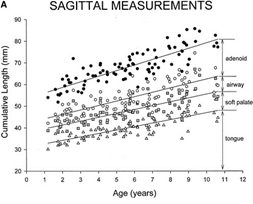
\includegraphics[width=0.5\linewidth]{images/length_of_airway_segments}
	\caption{Cumulative length of various airway segments}\label{length_of_airway_segments}
\end{figure}

\subsection{Advantages of process re-evaluation}
The advantages of the process re-creation have been touched on in the previous “Goal of the project” and “Requirements for a better process” sections. The new process should be easier to use than the old one, so that when new CT scans are provided, they can quickly be turned into viable models for study to broaden the available data set for studies done on sets of these models. This will also lead to a better understanding of various conditions through different age groups and genders.

The improved physical model will result in more accurate physical measurements; the focus on providing an easier rapid manufacturing process will result in more printable models that will expand the result set of any physical measurements

This work will lay further foundations in the area of upper airway modelling, further development could be based on it to expand on these advantages further.

\subsection{Outlook towards possible future use cases}
The upper airway does not only transport air to the lung but also plays an important part in speaking and singing. The models produced could be used to provide additional insight into these processes through simulation and testing of audio propagation. Several types of audio propagation could be studied, not only phonetic but also other processes such as snoring.

Snoring is a symptom of obstructive sleep apnea (OSA). During sleep, the upper airway may partially or completely collapse. It is a common disorder, with 9\% to 38\% of the general population suffering from it. It is also increasingly prevalent in older age groups with occurrence rates as high as 90\% in older men and 78\% in older women. Simulation using these models through Ansys and real-life testing by modification of physical models could provide valuable insight into the conditions inside the upper airways when symptoms occur.

Studying these symptoms in patients takes a considerable amount of time, manpower and patients willing to undergo study. With models created from one CT examination, the condition could be replicated much more rapidly, and conditions studied without patient involvement, leading to faster and more effortless findings on the topic. The advantages this process and these models bring for analysing OSA could be applied to many more similar conditions.

\chapter{Materials and Methods}

\section{Project structure, Work packages}

The process was split into three major parts, each handled by one of the team members. “Segmentation” would include taking the CT scans and creating a preliminary mesh of the upper airway through slicing, handled by Tamerlan Yusifov. “Physicalising” were to contain the processes that handled taking that mesh file and created a computer model from it to use for simulation and 3D printing. This would be a two-step process, involving first repairing the mesh generated by segmentation and then modifying it, mostly by adding two input- and output-ports for air to flow through. Finally, “Simulation”, handled by Samuel Henry Mba, was to take the model and run it through simulation software to simulate the flow and pressure at various stages inside.

\subsection{Schedule}

\begin{figure}[!htbp]
	\centering
	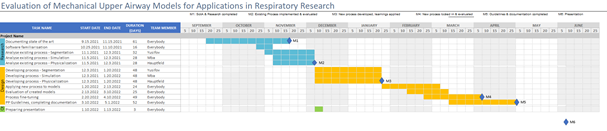
\includegraphics[width=1.0\linewidth]{images/schedule}
	\caption{Gantt chart depicting project scheduling}\label{schedule}
\end{figure}

\subsection{Initial Research}

The initial research would cover documenting state of the art information pertaining to this topic, such as previous work done, improvements to be made to that work and other surrounding information. Additionally, everyone was to do preliminary research into their work area with regards to the previous work, usable software and its availability, familiarization with that software and other similar topics.

\subsection{Evaluation of existing process}

The existing documentation regarding the process steps had to be evaluated by stepping through the existing instructions and software. In addition, the same scrutiny would be applied to relevant processes found during the research phase in case they contained any pertinent information. The process evaluation focused on three main aspects that would each focus on their own certain evaluation criteria. While model quality itself was not a specific criterion of any of these evaluations, it was hoped that a thorough evaluation of the individual criteria would have a positive effect on the model quality. At the very least, this method would establish documentation of existing processes and baseline learnings from which a new process could be created; this process could then be examined for possible model quality improvements.

\subsubsection{Documentation-based}

The \emph{documentation-based} evaluation was to look at the existing steps and information (such as settings, values) and verify both their informational content as well as their applicability to the range of provided CT imagery. For example, any vague wording that could lead to ambiguity regarding choices to be made during segmentation was to be identified for later rewriting based on learnings from this step. Purely informational content such as values to apply during segmentation was to be evaluated on the larger data set and either confirmed or marked for adjustment in the new process.

\subsubsection{Time-based}

For the \emph{time-based} evaluation, processes were to be split into segments and it would be analysed how much time was spent on these segments both in absolute and proportional (\% of the total process time) terms. This would allow identification of time sinks – actions in the process that took up excessive amounts of time and would require attempts at optimization. Time sinks could be identified as either computational (the execution time of a tool, a file parsing process) and human (requiring a lot of manual attention) types. Computational time sinks could only be mitigated by more processing power or use of different tools while human time sinks could stem from imprecise documentation or inefficient process steps.

\subsubsection{Issue-based}

During execution of a process, some error conditions may occur in the process due to mistakes or excessive variance in data like CT examinations. While, ideally, the documentation-based evaluation would iron out most flaws in the process that would lead to these error conditions the main process can’t account for all failure states. That is why, if any major oddities during trial of processes popped up, they were to be documented so a new process guide could include a description of them along with general advice on how to resolve the problem. That way, common mistakes can be more easily resolved, and the time and energy spent on resolvable situations may be reduced. 

\subsubsection{Points of concern}

For \emph{Segmentation}, the software 3D Slicer and the accompanying documented process had to be applied and evaluated.

\emph{Physicalising} required evaluation of the software MeshMixer and the associated process. No process or software regarding mesh modification or 3D printing was provided and no entirely relevant information was found during initial research. As such, none of this was analysed at this stage. This part of the process would have to be created from scratch.

In \emph{Simulation}, the Ansys simulation software was to be used on the model and the process again evaluated.

\subsection{Developing new process}

To develop the new process, knowledge from the initial research as well as the previous evaluation of the existing processes was to be taken to create a new and revised process. In the end, the new workflows should be easier to execute and applicable to a broader range of CT imagery.

\subsubsection{Segmentation}

To develop a new process for \emph{Segmentation}, the researched segmentation software (“3D Slicer” and “Materialise Mimics”) would be tested and evaluated for use in the process. Concrete criteria for evaluation would be availability, ease of use and resulting mesh quality with provided airway imagery.

The process for segmentation should consist of clear explanation of segmentation parameters and their effect on the produced mesh, including error states from the issue-based evaluation. Clear, sequential guidance should be given on how to proceed with segmentation, including suggested value ranges for the parameters (based on the documentation-based evaluation), with possible deviations based on special conditions (certain age groups, for example). In the end, the person applying the process should not have to use parameter values outside the specified ranges or spend excessive amounts of time on tedious manual processes (time-based evaluation) or adjusting values outside the defined ranges.

The new process would later be evaluated based on how well it could be applied to the 13 provided scans.

\subsubsection{Physicalising}

The process for \emph{Physicalising} would, as previously mentioned, be split into the groups “Mesh Repair” and “Mesh Modification”.

Software for Repair (MeshMixer, MeshLab and a custom mesh repair script) would be evaluated based on ability to produce a model usable for printing and analysing from a segmented mesh with minimal human intervention. At the end of the repair process the model should be completely hole-free while staying as true to the original mesh as possible and with as little time as possible having been invested. To that end, the provided tools in the software and their effectiveness would be evaluated as well as how many automation capabilities the software had. Full automation is a non-goal of this project, partial automation however could be beneficial to minimise required human post-processing. The learnings from these evaluations would be used to craft a new process suited to the software utilizing partial automation capabilities if existing as well as more detailed descriptions of possible fault conditions (faulty meshes) and the processes/tools used to remedy those conditions.

Modification software (OpenSCAD, Fusion360) were to be evaluated with regards to their ability to handle and modify imported mesh files, general ease of use, automatability and quality of resulting model. Additionally, it was to be evaluated if the resulting model would require another round of mesh repair – this was to be avoided if possible. The specific application for mesh modification in this case is the appending of physical input and output ports to the model used for attaching peripheral machinery to the printed model. Ideally, the process would result in a partly automated parametrized project file or script that would only require the user to place the ports in the correct positions. It would also be highly advantageous for the port models to be swappable with relative ease, as that would facilitate evaluation of various port geometry later in the project. With the development of this process, care had to be taken not to extend the scope of the automation to too high a degree, as this would both consume too much development time and make the process less universally applicable.

\subsubsection{Simulation}

Only the simulation software “Ansys”, used in the previous project, was to be considered. The software would be evaluated on the standard software evaluation parameters availability and ease of use. The simulation process was to be documented more thoroughly, with concise step-by-step instructions as well as documentation of possible erroneous configuration and steps on how to resolve them.

\subsection{Evaluation of new processes}

The new processes were to be evaluated on the provided CT sample imagery. During this, the process would be fine-tuned and subsequently “locked in” – after that point in time, no changes should be made. This would be a task for everyone.

\newpage
\subsection{Physical model testing}

During this phase, models printed during process evaluation would be tested in a physical setup. They would be included inside a pneumatic circuit, either having air pushed into them our vacuumed out of them, and the pressure and flows at the input and output of the airways would be measured. A diagram depicting a push-setup can be found in figure \ref{push-setup}.

\begin{figure}[!htbp]
	\centering
	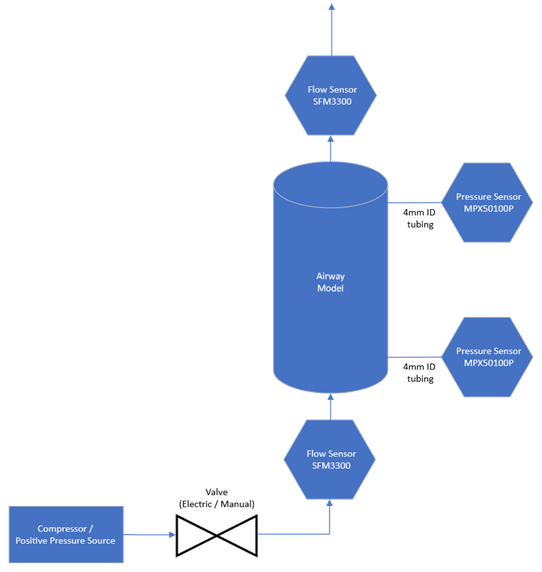
\includegraphics[width=.8\linewidth]{images/push-setup}
	\caption{Simplified push-configuration testing diagram}\label{push-setup}
\end{figure}

During this phase, various methods for connections between the model and the sensors and pressure sources would be tested and evaluated. Connections to the MPX50100P pressure sensors \cite{mpx5010} were previously accomplished using press-fit tubing of a 4mm inner diameter. The SFM3300 flow sensors \cite{sfm3300} featured standard female and male 22mm ventilator connections as defined by ISO5356-1:2004 \cite{iso5356}.

\subsection{Creation of process document guide}

Also, as a collective task, the new processes would be merged into a new process document that would contain all the new information in one document. This process document was to be created using the tool “mkdocs” to create both an easily navigable website and a PDF document for reference.

\section{Technical Documentation for software projects}

\subsubsection{Segmentation}
The following software was evaluated or incorporated (bold) into the segmentation process:

\begin{itemize}
	\item 3D Slicer
	\item Materialise Mimics
\end{itemize}
The following software was evaluated or incorporated (bold) into the physicalising process:

\subsubsection{Mesh Repair}

\begin{itemize}
	\item Autodesk MeshMixer
	\item MeshLab
	\item Custom repair script (Python)
\end{itemize}

\subsubsection{Mesh Modification}

\begin{itemize}
	\item OpenSCAD
	\item Autodesk Fusion 360
\end{itemize}

\section{Technical Documentation for hardware projects}

Additive rapid manufacturing technologies used include Fused Deposition Modelling (FDM) and Stereolithography (SLA).

\subsubsection{3D Printers, SLA}

\begin{itemize}
	\item Prusa SL1S
	\item Formlabs 2
\end{itemize}

\subsubsection{3D Printers, FDM}

\begin{itemize}
	\item Ultimaker 2+
	\item Prusa Mk3S+
\end{itemize}

During further work, this section will eventually be expanded to contain all the tested manufacturing materials, printer settings, ways of physical coupling and other machinery included in the physical testing process.

\section{Risk management}

The main risks of the existing process evaluation lie in the inability to identify any issues based on the proposed evaluation criteria. Furthermore, excessive amounts of time could be spent on trying to optimize process steps that are either a non-issue or exceedingly hard to optimize. To mitigate the risk of criteria failure, a more open analysis of the existing processes will be conducted if no issues can be identified through the evaluation criteria. To mitigate excessive time spent, only a certain amount of time within a maximum of a week is allowed to be spent on single identified issues.

\chapter{Results}

\section{Evaluation of existing processes and proposed changes}

\subsection{Segmentation}

\subsubsection{Software}

The software “Materialise Mimics” was planned to be evaluated for segmentation purposes, as it seemed to be more user friendly, however it was not available for free (license was required, no academic license available) so the choice fell on continuing use of the “3D Slicer” software.

\subsubsection{Evaluation of existing process sourced from the internet}

To get familiar with the mentioned software, YouTube tutorials \cite{yt-tutorials} were used as well as manuals from the internet. Firstly, CT scan data was installed from our source. Afterwards, instructions were carefully followed as in the tutorial. Initially, this involved pressing the “Load DICOM” button in the software and choosing the folder with the CT scans to load the data. Once this step was done, all CT scans were loaded to the software in different projections (in 3 different views, please refer to figure \ref{1-different-ct-projections}.

%\begin{figure}[!htbp]
%	\centering
%	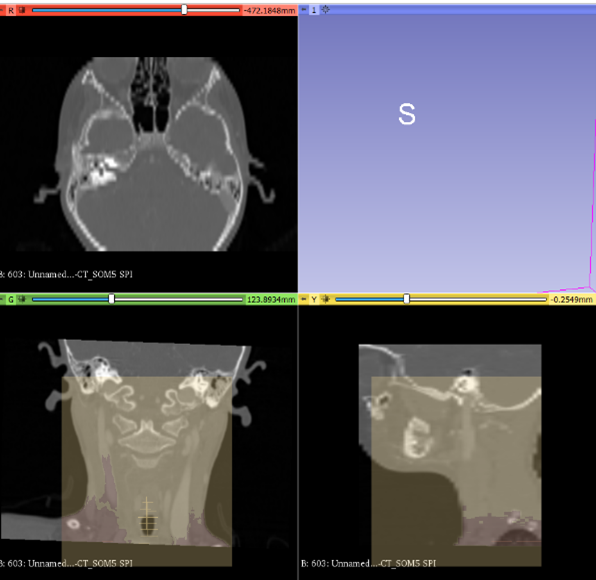
\includegraphics[width=.4\linewidth]{images/existing-evaluation/1-different-ct-projections}
%	\caption{3 different CT projections}\label{1-different-ct-projections}
%\end{figure}

After performing this step, one had to choose the “Segment Editor” option under the upper toolbar option. This mode allowed starting the segmentation process of the CT scans. After this, one had to choose the “Add” button and click it three times to have 3 different segments. They had to be renamed to simplify the downstream process: “Lung”, “Airways” and “Other”. Initial segmentations are performed on the “Lung” part, once this option is chosen, the “Paint” mode had to be selected. This mode allows circling of the region of interest to segment. For lungs, the black hollow region on the CT scans (this region refers to the lungs) has to be chosen. The following mode “Pain” had to be performed for the 2 other segment options -”Airways” and “Other”. The most difficult part was “painting” the airways, as it was extremely difficult to select in the CT scans. To segment airways on the CT scans, one had to select the circular black hollow region in the center of the CT scans – “Airways”. The “Other” segment refers to the lining of the lungs that also had to be accounted for by encircling. The procedure can be seen illustrated in figure \ref{2-segmentation-procedure}. 

%\begin{figure}[!htbp]
%	\centering
%	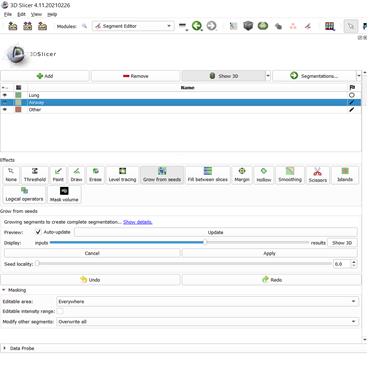
\includegraphics[width=.4\linewidth]{images/existing-evaluation/2-segmentation-procedure}
%	\caption{Segmentation procedure}\label{2-segmentation-procedure}
%\end{figure}
\begin{figure}[!htb]
	\begin{minipage}{0.48\textwidth}
		\centering
		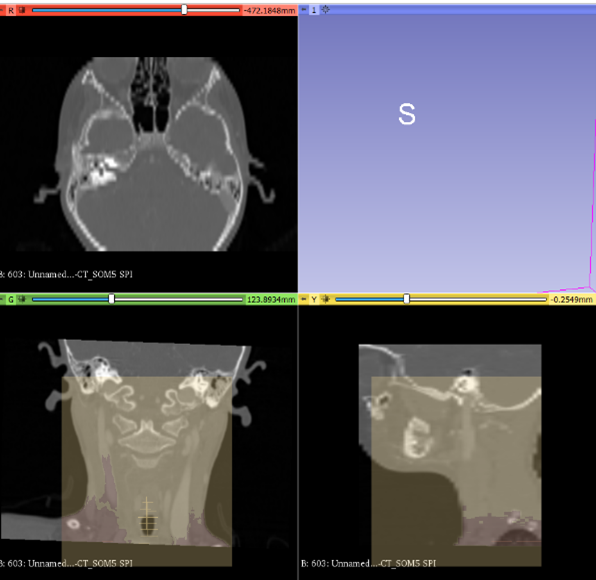
\includegraphics[width=.7\linewidth]{images/existing-evaluation/1-different-ct-projections}
		\caption{3 different CT projections}\label{1-different-ct-projections}
	\end{minipage}\hfill
	\begin{minipage}{0.48\textwidth}
		\centering
		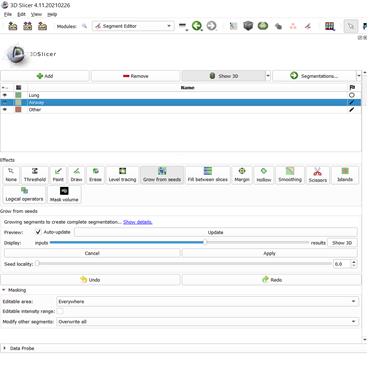
\includegraphics[width=.7\linewidth]{images/existing-evaluation/2-segmentation-procedure}
		\caption{Segmentation procedure}\label{2-segmentation-procedure}
	\end{minipage}
\end{figure}

After initializing the above-mentioned steps, one had to choose the effect “grow from seeds”, also selecting “everywhere” and “overwrite all options” under “editable area” and “modify another segment” respectively. The following procedure allows optimizing the 3D model afterwards. After these steps are performed, one must choose option “Initialize” to start the process of segmentation of the model.  Once this step is done, one has to choose the option “Show 3D” to obtain the model of the right side of the screen, this step might take a few minutes. 
Unfortunately, obtained results at this moment do not look any near to the desired results (please refer to the figure \ref{3-example-of-how-should-look}). The main reason behind this is the fact that the vast majority of tutorials and online guides from the source are working with already existing data from the 3D slicer, thus it is very straightforward to choose desired regions of interest from the CT scans (please refer to figure ref{4-data-used-in-the-source}). In a contrast, it was very difficult to select / ”paint” the desired region in the given CT scans, due to the fact that the provided CT scans were of the whole upper part of the body, compared to the CT scans in all of the tutorials that are solely of the chest part of the body, which makes it very easy to select the desired parts. 

\begin{figure}[!htbp]
	\centering
	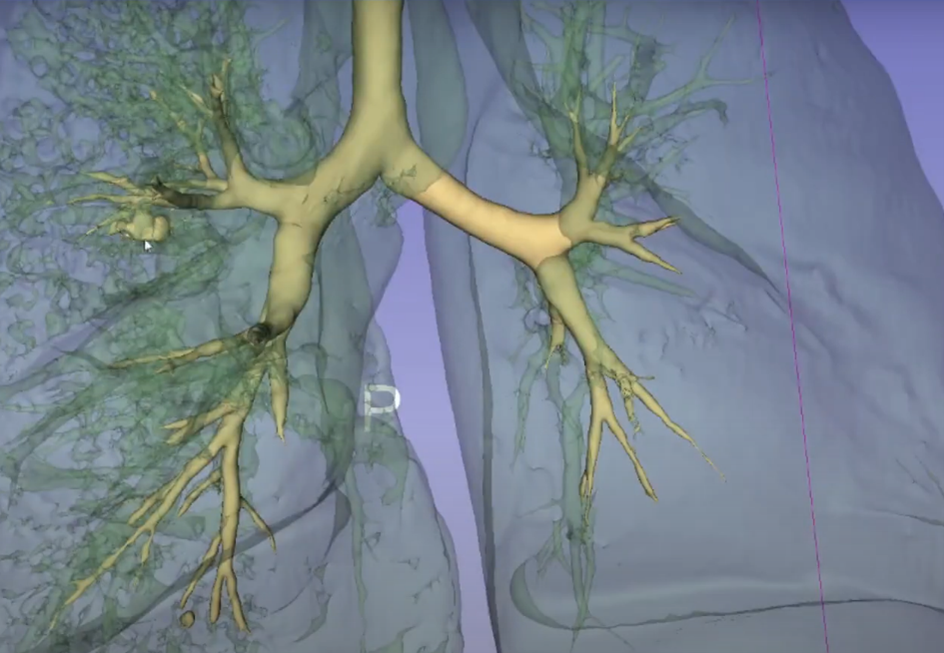
\includegraphics[width=.4\linewidth]{images/existing-evaluation/3-example-of-how-should-look}
	\caption{Example of how the model should look, taken from an online source}\label{3-example-of-how-should-look}
\end{figure}

\begin{figure}[!htbp]
	\centering
	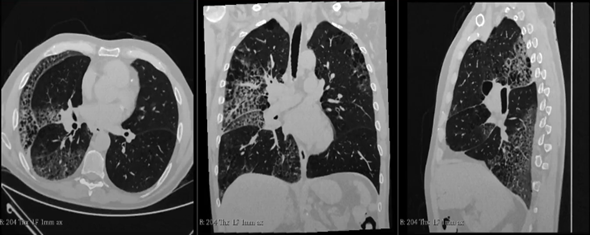
\includegraphics[width=.4\linewidth]{images/existing-evaluation/4-data-used-in-the-source}
	\caption{Data that was used in the source, where lungs and airways can be clearly seen}\label{4-data-used-in-the-source}
\end{figure}

To get the model as close as possible to desired result, the process of “painting” the desired regions of the CT scans had to be studied more closely in order to make sure to select all the regions. In case of the model not conforming to the standard closely enough, manual “painting” must be used as well. Please, refer to figure \ref{5-intermediate-model} to see the model that was obtained so far using the software. 

\begin{figure}[!htbp]
	\centering
	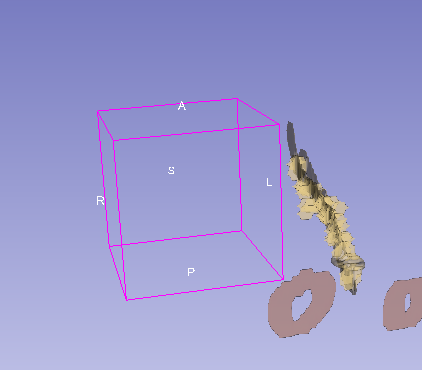
\includegraphics[width=.4\linewidth]{images/existing-evaluation/5-intermediate-model}
	\caption{Intermediate model, work-in-progress}\label{5-intermediate-model}
\end{figure}

Another improvement that has to be made is to do with the software, more research must be conducted in order to understand the full functionality and possibilities of the given software. Moreover, one may consider using the “Cropping” mode to get rid of the parts of CT scan that are unwanted.

\subsubsection{Evaluation of existing process from previous group}

Most of the existing documentation from the previous group handled the segmentation process, there were multiple pages to evaluate.

The following \textbf{\emph{documentation-based}} issues were identified in the existing process:

\begin{itemize}
	\item The import process into 3D slicer is not documented. The data arrived in DICOM format with a special tool and a proprietary metadata format. The import process was not trivial and should be covered in the future.
	\item The selection of series and by which criteria a base series for segmentation should be selected was barely, if at all mentioned
	\item Adding of segments and their relevance should be briefly described, with references to Slicer documentation
	\item The mechanisms behind the “Grow from seeds” tool and the usage of its 3D view to evaluate the result is poorly documented – again, provide a short description with references
	\item Non-trivial export process to STL is not described, multiple parameters can be adjusted
\end{itemize}

Furthermore, the given range of threshold values for selection of air segments was evaluated. These should not differ majorly (within 10-15\%) between different examinations with the same machine. Since the CT machine was not identifiable, the values are categorized by the anonymous patient IDs of the provided samples.

\begin{table}[!htbp]
	\centering
	\caption{Applied threshold values in segmentation}\label{tab-threshold}
	\begin{tabular}{| p{0.3\linewidth} | p{0.3\linewidth} |}\hline
		Patient ID & Threshold \\\hline
		0181172089 & -221 \\
		0190544287 & -240 \\
		0190667317 & -220 \\\hline
	\end{tabular}
\end{table}

For the \textbf{\emph{time-based evaluation}}, a later segmentation run of patient 0190544287 was recorded by the same person on two different systems (PC and Notebook) and the time spent on each segment identified. The total time distribution of segmentation is as follows in figure \ref{segmentation-time-proportions}.

\begin{figure}[!htbp]
	\centering
	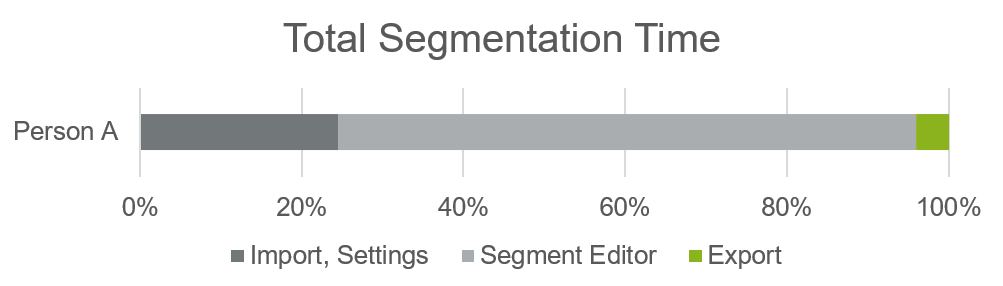
\includegraphics[width=.8\linewidth]{images/segmentation-time-proportions}
	\caption{Segmentation Time Proportions}\label{segmentation-time-proportions}
\end{figure}

As is evident of the proportions graph, the vast majority of time is spent in the segment editor. Since it takes up such a major portion of the time, this segment was again split into smaller segments to identify time sinks that could be optimized within it.

\begin{figure}[!htbp]
	\centering
	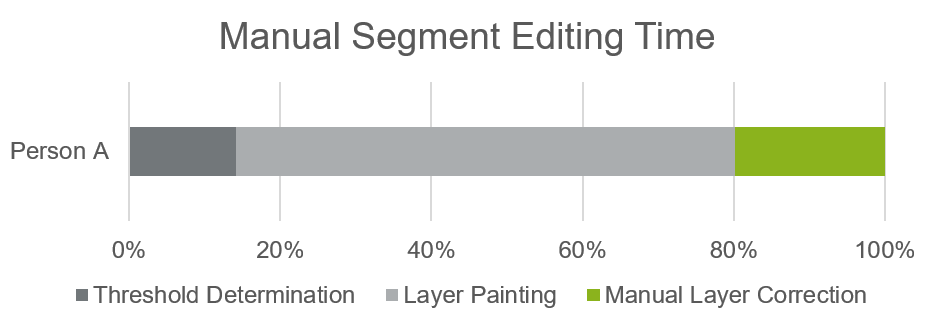
\includegraphics[width=.8\linewidth]{images/manual-segment-editing-proportions}
	\caption{Manual Segment Editing Proportions}\label{manual-segment-editing-proportions}
\end{figure}

Again, it is clear from the graph in figure \ref{manual-segment-editing-proportions} that most of the time spent on segmentation is in the “layer painting” phase, where the air in airways is painted on multiple layers to provide a basis for the “grow from seeds” function to later connect these markings to a full airway segmentation.

The biggest measure to reduce time spent on this phase would be to provide guidelines on which areas require the most manual attention (the most manually painted layers) due to complex structures and which require very little human intervention and can be mostly segmented by the computer / the tool.

\begin{figure}[!htbp]
	\centering
	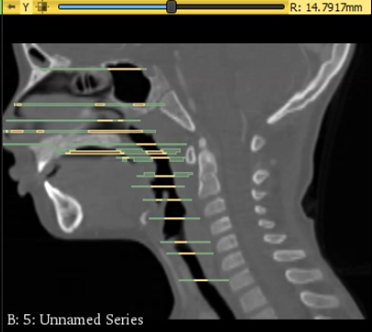
\includegraphics[width=.4\linewidth]{images/segmentation-area-complexity}
	\caption{Segmentation Area Complexity}\label{segmentation-area-complexity}
\end{figure}

As can be seen in figure \ref{segmentation-area-complexity}, the most complex area is around the nasopharynx and nasal cavity as well as the oropharynx while the larynx is a comparatively simple tube. The upper marked area requires significantly more manual work than the lower one – spending time on the lower area is mostly wasted and future documentation should reflect that.

Furthermore, it should be documented that the size of the brush used for manual painting can be adjusted – this greatly reduces time spent on layers with more complex geometry.

During research, it was discovered that experimental segmentation tools exist for Slicer that were demonstrated to be a very fast method for segmenting areas with good contrast \cite{fast-marching}. Being air filled cavities, the upper airways would provide such contrast to the surrounding bones and tissue. However, the evaluation could not be completed because the experimental tools would often not work, citing various error messages. Sometimes they crashed or hung the slicer Software entirely. Purely based on the documentation on them that was researched, they seem an interesting prospect and should be revisited when they have reached more maturity.

Lastly, some of the tool performance was compared between a PC and a Laptop processor; the time savings from a faster processor turned out negligible unless a tool had to be used many times over. The most computationally demanding tools (Import \& Grow from seeds) only came to use one time in the process, as such the computational time sinks can be ignored.

\begin{figure}[!htbp]
	\centering
	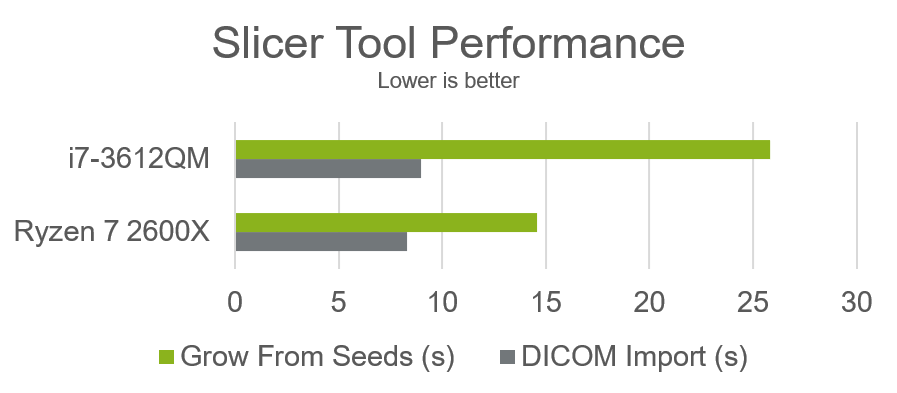
\includegraphics[width=.8\linewidth]{images/slicer-tool-performance}
	\caption{Slicer Tool Performance}\label{slicer-tool-performance}
\end{figure}

An error state that could be identified during \textbf{\emph{issue-based process evaluation}} was that a negative 3D mesh surrounding the desired airway mesh appeared after the “grow from seeds” function was applied.  The state is illustrated in figure \ref{error-state-negative-mesh}.

\begin{figure}[!htbp]
	\centering
	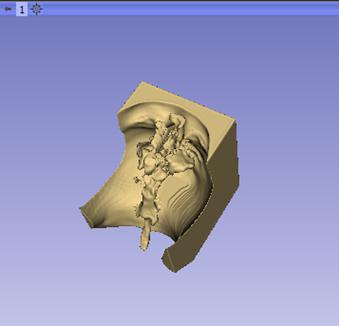
\includegraphics[width=.5\linewidth]{images/error-state-negative-mesh}
	\caption{Error State: Negative Mesh}\label{error-state-negative-mesh}
\end{figure}

This can be remedied by adding an additional background layer outside patient physiology. Alternatively, these parts can be cut off using the cutting tool of Slicer. No documentation on efficient use of the cutting tool within the airway modelling context was provided in the previous document, the cutting tool itself was found to only be useful as a last resort. Nevertheless, experience with the cutting tool especially with regards to airway modelling should be documented and Slicer documentation referenced to save time for other users encountering this condition.

\newpage
\subsection{Physicalising (Mesh repair \& modification)}

Only the part of mesh repair was explained in the existing process so only that can be evaluated. The repair was conducted using AutoDesk MeshMixer and its “Fix Holes” functionality.

This was found to be well working in initial testing, but the process did not include any documentation beyond “use that tool”. If any fault conditions are found in further testing, the existing process guide would provide no guidance in that regard and would leave process users researching problems on their own. Additionally, the process of opening MeshMixer just to push a button was cumbersome and MeshMixer provided no functionality to automate this process via any means. Additional software would have to be evaluated and if it could provide fixing abilities on a similar level while also being automatable, it would be preferrable to use them instead. A short guide on common issues during mesh repair should also be developed, in case problems arise with a wider set of data.

\subsection{Simulation}

Ansys is an engineering simulation and 3D design software which delivers product modelling solutions, it is used to simulate computer models of structures, electronics or machine components for analysing strength, toughness, elasticity, temperature distribution, electromagnetism, fluid flow, and other attributes. 

After obtaining the model from the previous parts in the process, Ansys Software was to be used for simulating flow and pressure through the model. Firstly, the Ansys Spaceclaim software has to be used for editing, repairs and to simplify the model for simulation before the model will be exported for meshing through Ansys Meshing. Since meshing typically consumes a significant amount of time it takes to get simulation results, Ansys Meshing helps by making better and more automated meshing tools. 
With this tool zones and inflations can be added to generate a secondary mesh which has more compatibility with the Ansys simulation. And lastly this model will be imported to Ansys Fluent for measurements through simulation.

Ansys is a group of software’s which allows you to perform different forms of Engineering simulation. The software turned out to be quite difficult concerning ease of use and the vast array of different software that needed to be used to achieve a good simulation result presented a steep learning curve. 

\newpage
\section{Development of new process}

\subsection{Physicalising}

The physicalising process was split into two parts. Mesh repair deals with software and processes evaluated regarding the conversion of mesh data from segmentation into viable models by patching holes and other irregularities and modification looks at software and processes to do with adding peripheral attachment mechanisms (ports) to the model by modifying the existing mesh/model.

\subsubsection{Software}

For \textbf{\emph{repair}}, three software products were evaluated based on the criteria provided in “methods”. The first is Autodesk MeshMixer, used in the previous work and a proprietary, albeit free-to-use, Autodesk product. The second was MeshLab, an open-source software with certain automation qualities. Lastly, the possibility of using a completely custom script was investigated

\subsubsection{Hollowing}

For both simulated and physical flows through a model it would need to be hollowed out. As the mesh resulting from segmentation is a solid model of the air-filled cavities of the upper airways, this step could also be called “turning the model inside out”. This process was not documented at all in the information from the previous groups and would therefore need to be tested and documented anew. It is of vital importance that the space inside the geometry resulting from this step represents the geometry of the air-filled cavities exactly – otherwise the representation would be inaccurate. The new walls need to be generated on the outside of the existing geometry. Figure \ref{hollowing-illustration} illustrates the process and these concerns.

\begin{figure}[!htbp]
	\centering
	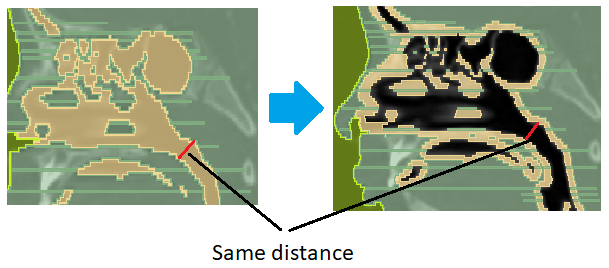
\includegraphics[width=.8\linewidth]{images/hollowing-illustration}
	\caption{Hollowing Illustration}\label{hollowing-illustration}
\end{figure}

Both 3D slicer (used for figure \ref{hollowing-illustration} above) and MeshLab support this kind of hollowing of geometry. 3D slicers hollowing feature proved adequately functional but issue-prone, and the mesh required significant correction in MeshLab anyway, making the case for moving the entire process there. MeshLab hollowing functionality has yet to be evaluated.

\chapter{Discussion}

\section{Process Evaluation}
The three-concern methodology for process evaluation proved efficient in practice and easy to apply. While some additional concern for quality of the result should be added in the future the identified issues and their remedies should already be an improvement to the process and provide a solid foundation for future development.  While criteria-based evaluation has yet to be applied to the improvements, in preliminary testing they showed promise for streamlining the process and easing the workload for processing of many examinations, especially with regards to segmentation.

\newpage
\chapter{References}

\printbibliography[heading=none]

\clearpage
% Das Abbildungsverzeichnis
\listoffigures

% Das Tabellenverzeichnis
\listoftables

% Das Quellcodeverzeichnis
\listofcode

\end{document}
